%%%%%%%%%%%%%%%%%%%%%%%%%%%%%%%%%%%%%%%%%%%%%%%%%%%%%%%%%%%%%%%%%%%%%%%%%%%

\documentclass[a4paper,oneside,12pt]{article}
\usepackage{mystyle}

\begin{document}

\title{\Large\bf Linear functions}
\author{%%
  Minh Van Nguyen \\
  \url{mvngu@gmx.com}
}
\date{\today}
\maketitle


%%%%%%%%%%%%%%%%%%%%%%%%%%%%%%%%%%%%%%%%%%%%%%%%%%%%%%%%%%%%%%%%%%%%%%%%%%%

\section{General form}
\label{sec:general_form}

A \emph{linear function} is an expression of the form
%%
\begin{equation}
\label{eqn:linear_function_general}
f(x)
=
ax + b.
\end{equation}
%%
The numbers $a$ and $b$ are fixed real numbers such that $a \neq 0$,
while $x$ is a variable that can be any real number.  What does the
function $f(x)$ look like?

As an example, set $a = b = 1$ in
\Equation{eqn:linear_function_general} so that you have
$f(x) = x + 1$.  The graph of $f(x) = x + 1$ is a straight line that
passes through the point $A = \tuple{-1}{0}$ on the $x$-axis and the
point $B = \tuple{0}{1}$ on the $y$-axis.  How were the coordinates of
$A$ and $B$ calculated?  For the point $A$, you set $f(x) = 0$ and
solve the equation $0 = x + 1$ for $x$ to get $x = -1$.  The
$x$-coordinate of $A$ is $-1$ and the $y$-coordinate is $0$.  For the
point $B$, you set $x = 0$ and solve the equation $y = 0 + 1$ for $y$
to obtain $y = 1$.  Then $B$ has $x$-coordinate $0$ and $y$-coordinate
$1$.  Plot the points $A$ and $B$, then draw a straight line through
those two points to produce the graph in \Figure{fig:plot_x_+_1}.

\begin{figure}[!htbp]
\centering
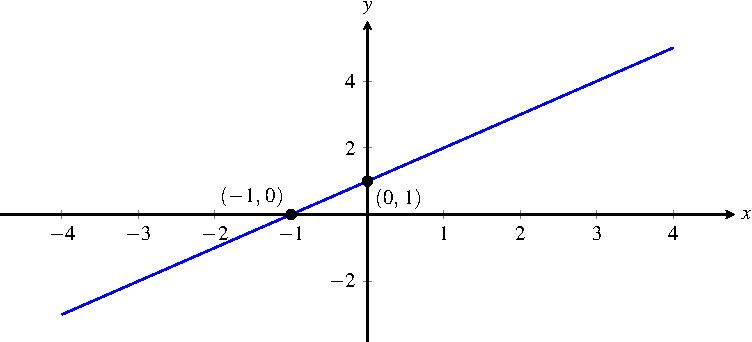
\includegraphics[scale=1]{image/06/a-1-b-1.pdf}
\caption{%%
  A graph of the function $f(x) = x + 1$.
}
\label{fig:plot_x_+_1}
\end{figure}

In general, how would you draw the graph of the
\Function{eqn:linear_function_general}?  As in the example above, you
want to determine two different points of the function $f(x)$.  A
common way to do so is as follows.  You set $f(x) = 0$ and determine
the point $A = \tuple{\alpha}{0}$, where $x = \alpha$ is obtained by
solving $f(x) = 0$ for $x$.  You then set $x = 0$ and determine the
point $B = \tuple{0}{\beta}$, where $\beta = f(0)$.  Plot the points
$A$ and $B$, then draw a straight line through those two points.  The
result is a graph of the \Function{eqn:linear_function_general}.  The
point $A = \tuple{\alpha}{0}$ is called the $x$-intercept because this
is the point where the graph of $f(x) = ax + b$ intersects the
$x$-axis.  Similarly, the point $B = \tuple{0}{\beta}$ is the
$y$-intercept because it is the point where the graph of $f(x)$
intersects the $y$-axis.  Let's put the above strategy into practice.

\begin{example}
Suppose in the equation $f(x) = ax + b$ you set $a = 2$ and
$b = -1 / 2$.  Draw a graph of the function
$f(x) = 2x - \frac{1}{2}$.
\end{example}

\begin{solution}
To obtain the $x$-intercept $A$, you set $f(x) = 0$ and solve the
equation $0 = 2x - \frac{1}{2}$ for $x$.  The latter equation can be
written as $2x = \frac{1}{2}$ and dividing both sides by $2$ shows
that
%%
\begin{align*}
x
&=
\frac{1}{2} \div 2 \\[4pt]
&=
\frac{1}{2} \times \frac{1}{2} \\[4pt]
&=
\frac{1}{4}.
\end{align*}
%%
In other words, the $x$-intercept has coordinates
$A = \tuple{\frac{1}{4}}{0}$.  The coordinates of the $y$-intercept
$B$ are determined by first setting $x = 0$.  You then solve the
equation $y = 2 \times 0 - \frac{1}{2}$ for $y$.  The latter equation
can be written as
%%
\begin{align*}
y
&=
2 \times 0 - \frac{1}{2} \\[4pt]
&=
0 - \frac{1}{2} \\[4pt]
&=
-\frac{1}{2}
\end{align*}
%%
and you have the $y$-intercept $B = \tuple{0}{-\frac{1}{2}}$.  Plot
the points $A$ and $B$ and draw a straight line through the two points
to produce the graph in \Figure{fig:plot_2x_minus_half}.
\end{solution}

\begin{figure}[!htbp]
\centering
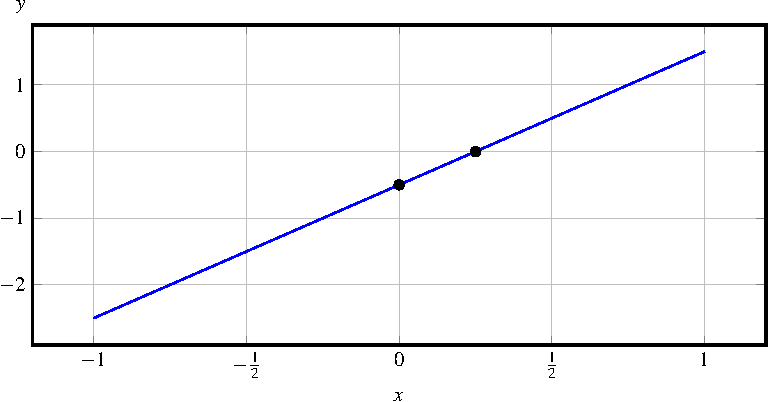
\includegraphics[scale=1]{image/06/a-2-b-minus-half.pdf}
\caption{%%
  A graph of the function $f(x) = 2x - \frac{1}{2}$.
}
\label{fig:plot_2x_minus_half}
\end{figure}

\begin{exercise}
Draw a graph of the function $f(x) = 2x - 2$.
\end{exercise}

\ifbool{showSolution}{
\begin{solution}
You want two different points $A$ and $B$ of the function
$f(x) = 2x - 2$.  A graph of the function is obtained by drawing a
straight line through those two points.  First, you set $f(x) = 0$ and
solve the equation $0 = 2x - 2$ for $x$.  You can write the latter
equation as $2x = 2$ and dividing both sides by $2$ shows that
$x = 1$.  Thus you have the point $A = \tuple{1}{0}$.  Second, you set
$x = 0$ and solve the equation $y = 2 \times 0 - 2$ for $y$.  Write
the last equation as $y = 0 - 2$ and you see that $y = -2$.  Thus you
have the point $B = \tuple{0}{-2}$.  Plot the two points $A$ and $B$,
draw a straight line through those two points, and you have the graph
in \Figure{fig:plot_2x_minus_2}.

\begin{figure}[!htbp]
\centering
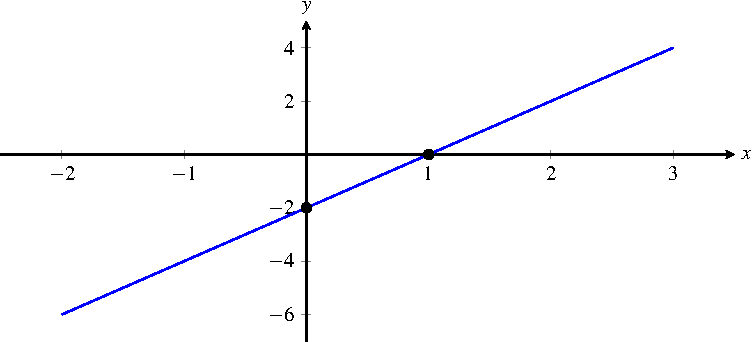
\includegraphics[scale=1]{image/06/a-2-b-minus-2.pdf}
\caption{%%
  A graph of the function $f(x) = 2x - 2$.
}
\label{fig:plot_2x_minus_2}
\end{figure}
\end{solution}
}{}

\begin{exercise}
Draw a graph of the function $f(x) = 3x + \frac{1}{2}$.
\end{exercise}

\ifbool{showSolution}{
\begin{solution}
Determine two points of the function $f(x)$ and draw a straight line
through those two points to produce a graph of the function.  For the
first point, set $f(x) = 0$ and solve the equation
$0 = 3x + \frac{1}{2}$ for $x$.  The latter equation can be written as
$3x = -\frac{1}{2}$.  Multiply both sides by $\frac{1}{3}$ to see that
$x = -\frac{1}{2} \times \frac{1}{3} = -1 / 6$ and you have the point
$A = \tuple{-\frac{1}{6}}{0}$.  For the second point, set $x = 0$ and
solve the equation $y = 3 \times 0 + \frac{1}{2}$ for $y$.  The last
equation can be written as $y = 1 / 2$ and you have the point
$B = \tuple{0}{\frac{1}{2}}$.  Plot the two points and draw a straight
line through those two points to produce the graph in
\Figure{fig:plot_3x_half}.

\begin{figure}[!htbp]
\centering
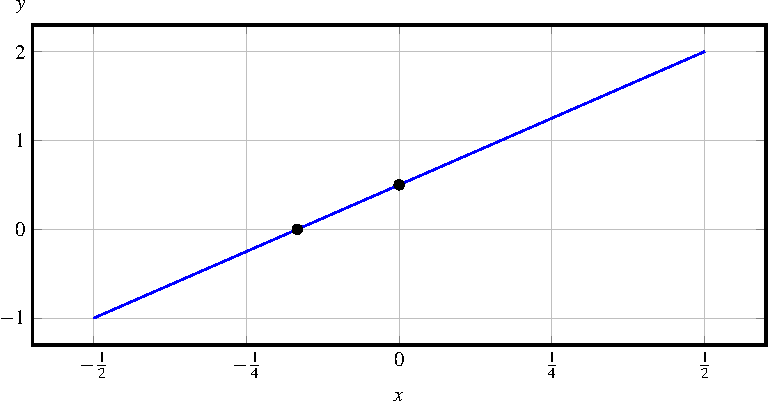
\includegraphics[scale=1]{image/06/a-3-b-half.pdf}
\caption{%%
  A graph of the function $f(x) = 3x + \frac{1}{2}$.
}
\label{fig:plot_3x_half}
\end{figure}
\end{solution}
}{}


%%%%%%%%%%%%%%%%%%%%%%%%%%%%%%%%%%%%%%%%%%%%%%%%%%%%%%%%%%%%%%%%%%%%%%%%%%%

\section{Special cases}

In the function $f(x) = ax + b$, suppose you set $a = 0$ and end up
with $f(x) = b$.  The function $f(x) = b$ states that no matter what
the value of $x$ is you will always get $y = b$.  For this reason, the
function $f(x) = b$ is called a \emph{constant function}.  The graph
of the constant function $f(x) = b$ is a horizontal line through the
point $b$ on the $y$-axis and this horizontal line is parallel to the
$x$-axis.  See \Figure{fig:constant_functions} for the examples of
$b = 2$ and $b = -3$.

\begin{figure}[!htbp]
\centering
\subfigure[]{
  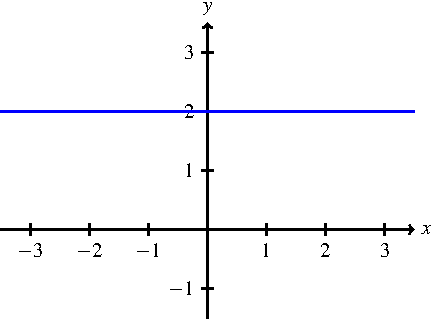
\includegraphics[scale=0.8]{image/06/a-0-b-2.pdf}
}
%%
\qquad
%%
\subfigure[]{
  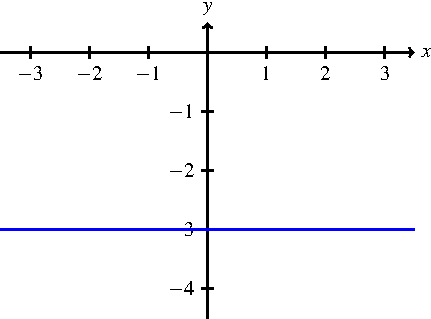
\includegraphics[scale=0.8]{image/06/a-0-b-minus-3.pdf}
}
\caption{%%
  Plots of the constant functions (a)~$f(x) = 2$ and
  (b)~$f(x) = -3$.
}
\label{fig:constant_functions}
\end{figure}

\begin{exercise}
Describe the function $f(x) = -1/2$ and draw its graph.
\end{exercise}

\ifbool{showSolution}{
\begin{solution}
The expression $f(x) = -1/2$ is a constant function.  Its graph is a
horizontal line through the point $-1/2$ on the $y$-axis and this line
is parallel to the $x$-axis.
\Figure{fig:constant_function_minus_half} shows a graph of the
function $f(x)$.
%%
\begin{figure}[!htbp]
\centering
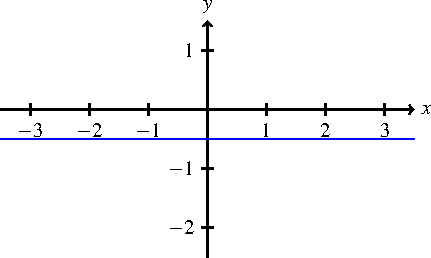
\includegraphics[scale=1]{image/06/a-0-b-minus-half.pdf}
\caption{%%
  A graph of the constant function $f(x) = -1/2$.
}
\label{fig:constant_function_minus_half}
\end{figure}
\end{solution}
}{}

\begin{exercise}
\label{ex:constant_function_zero}
Describe the graph of the expression $f(x) = 0$.
\end{exercise}

\ifbool{showSolution}{
\begin{solution}
The expression $f(x) = 0$ is a constant function whose graph is a
horizontal line through the point $0$ on the $y$-axis.  In other
words, the function $f(x) = 0$ describes the $x$-axis.
\end{solution}
}{}

Now consider the case of $b = 0$ in the function $f(x) = ax + b$.
What you end up with is the function $f(x) = ax$.  If you also have
$a = 0$, then $f(x)$ is reduced to the function in
\Exercise{ex:constant_function_zero}.  Otherwise assume that
$a \neq 0$.  What does the graph of $f(x) = ax$ look like?

Let's use the strategy from \Section{sec:general_form} to graph
$f(x) = ax$.  Set $f(x) = 0$ and solving the equation $0 = ax$ for $x$
results in $x = 0$.  The $x$-intercept has coordinates
$A = \tuple{0}{0}$.  Next, set $x = 0$ and solving the equation
$y = a \times 0$ for $y$ shows that $y = 0$.  The $y$-intercept is
$B = \tuple{0}{0}$.  Both of $A$ and $B$ are the same point and that
point is the origin.  You need another way to determine a second and
different point of the function $f(x) = ax$.

Instead of setting $x = 0$, you can try setting $x = 1$.  Simplify the
equation $y = a \times 1$ and you obtain $y = a$.  Hence the
second~(and different) point is $\tuple{1}{a}$.  In other words, if
$a \neq 0$ then the graph of $f(x) = ax$ is a straight line that
passes through the origin.  \Figure{fig:function_ax_positive_rational}
shows some graphs of $f(x) = ax$, where $a$ is a positive real number
that is at most $1$, i.e.~$0 < a \leq 1$.
\Figure{fig:function_ax_positive_at_least_one} shows some graphs of
$f(x) = ax$ for the case where $a \geq 1$.  Notice that in both of
these figures, the graphs of $f(x) = ax$ pass through the point
$\tuple{0}{0}$.

\begin{figure}[!htbp]
\centering
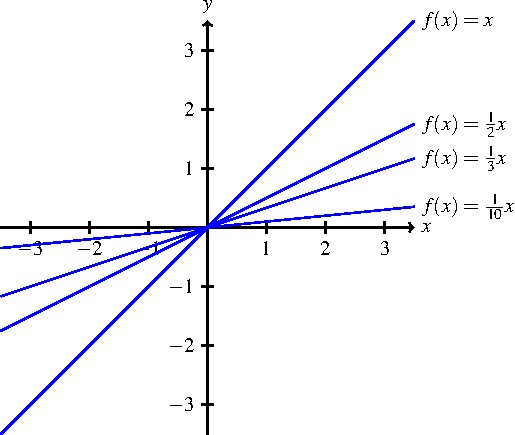
\includegraphics[scale=1]{image/06/ax-small.pdf}
\caption{%%
  Graphs of the function $f(x) = ax$ for various values of $a$, where
  it is assumed that $0 < a \leq 1$.  As the value of $a$ becomes
  smaller and smaller, the graph of $f(x) = ax$ becomes more and more
  like a horizontal line.
}
\label{fig:function_ax_positive_rational}
\end{figure}

\begin{figure}[!htbp]
\centering
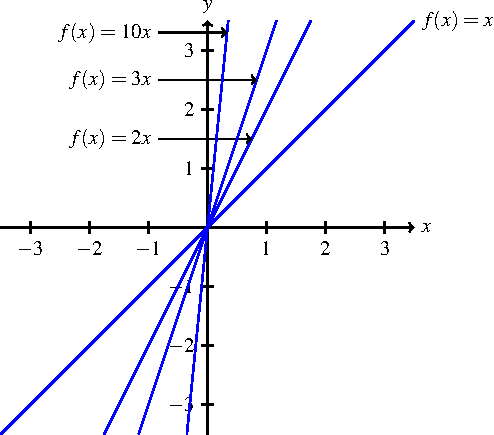
\includegraphics[scale=1]{image/06/ax-large.pdf}
\caption{%%
  Graphs of the function $f(x) = ax$ for various values of $a$, where
  $a \geq 1$.  As the value of $a$ becomes larger and larger, the
  graph of $f(x) = ax$ becomes steeper and steeper like a vertical
  line.
}
\label{fig:function_ax_positive_at_least_one}
\end{figure}

\begin{exercise}
Describe the graphs of the function $f(x) = ax$, where the factor $a$
takes on the values
$a = \quadruple{-\frac{1}{10}}{-\frac{1}{3}}{-\frac{1}{2}}{-1}$.
\end{exercise}

\ifbool{showSolution}{
\begin{solution}
\Figure{fig:graph_ax_a_negative_between_0_minus_1} shows the graphs of
$f(x) = ax$ for the above given values of $a$.  Note that
$-1 \leq a < 0$.  As $a$ becomes larger and larger and approaches zero,
the graph of $f(x) = ax$ becomes more and more like a horizontal line.

\begin{figure}[!htbp]
\centering
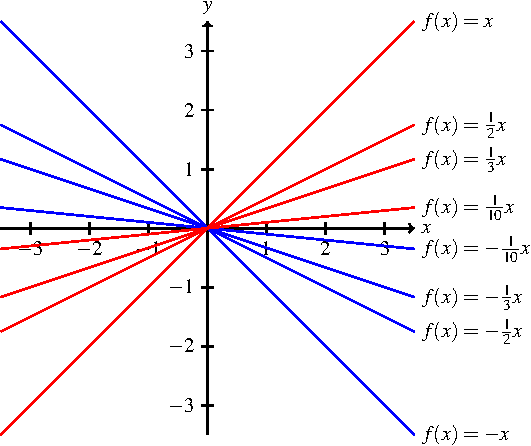
\includegraphics[scale=1]{image/06/ax-small-negative.pdf}
\caption{%%
  The blue lines are graphs of the function $f(x) = ax$, where $a$ has
  the values
  $a = \quadruple{-\frac{1}{10}}{-\frac{1}{3}}{-\frac{1}{2}}{-1}$.
  The red lines are reflections about the $x$-axis of the blue lines.
}
\label{fig:graph_ax_a_negative_between_0_minus_1}
\end{figure}
\end{solution}
}{}

\begin{exercise}
Describe the graphs of the function $f(x) = ax$, where the factor $a$
takes on the values $a = \quadruple{-1}{-2}{-3}{-10}$.
\end{exercise}

\ifbool{showSolution}{
\begin{solution}
\Figure{fig:graph_ax_a_negative_less_than_1} shows the graphs of
$f(x) = ax$ for the above given values of $a$.  Starting from
$a = -1$, as $a$ becomes smaller and smaller, the graph of
$f(x) = ax$ becomes steeper and steeper like a vertical line.

\begin{figure}[!htbp]
\centering
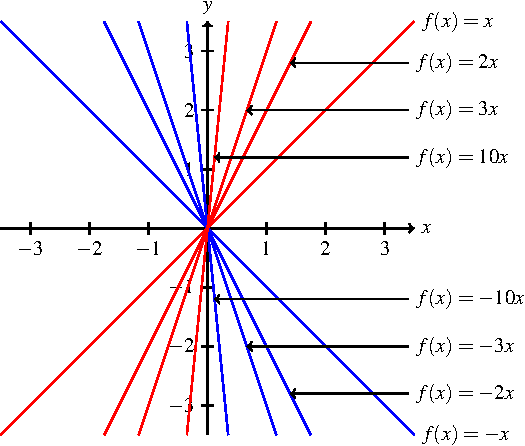
\includegraphics[scale=1]{image/06/ax-large-negative.pdf}
\caption{%%
  The blue lines are graphs of the function $f(x) = ax$, where $a$ has
  the values $a = \quadruple{-1}{-2}{-3}{-10}$.  The red lines are
  reflections about the $x$-axis of the blue lines.
}
\label{fig:graph_ax_a_negative_less_than_1}
\end{figure}
\end{solution}
}{}


%%%%%%%%%%%%%%%%%%%%%%%%%%%%%%%%%%%%%%%%%%%%%%%%%%%%%%%%%%%%%%%%%%%%%%%%%%%

\section{Table of values}

A linear function $f(x) = ax + b$ can also be represented as a table
of values.  The table has two columns.  The left column specifies a
number of values for $x$ and the right column gives the corresponding
values for $f(x)$.  For example, \Table{tab:function_values_a_2_b_1}
shows some values of the function $f(x) = 2x + 1$.  For $x = -3$ you
have the value $f(-3) = 2(-3) + 1 = -6 + 1 = -5$.  For $x = 1$ you
have $f(1) = 2 \times 1 + 1 = 3$.  And so on.

\begin{table}[!htbp]
\centering
\begin{tabular}{rr} \toprule
$x$  & $f(x)$ \\\midrule
$-3$ & $-5$   \\[6pt]
$-2$ & $-3$   \\[6pt]
$-1$ & $-1$   \\[6pt]
$0$  & $1$    \\[6pt]
$1$  & $3$    \\[6pt]
$2$  & $5$    \\[6pt]
$3$  & $7$    \\\bottomrule
\end{tabular}

\caption{%%
  Some specific values of the function $f(x) = 2x + 1$.
}
\label{tab:function_values_a_2_b_1}
\end{table}

\begin{exercise}
Provide a table of values for the function $f(x) = \frac{x}{2} + 2$ at
the values of $x = \quintuple{-2}{-1}{0}{1}{2}$.
\end{exercise}

\ifbool{showSolution}{
\begin{solution}
See \Table{tab:function_values_a_half_b_2}.

\begin{table}[!htbp]
\centering
\begin{tabular}{cc} \toprule
$x$  & $f(x)$  \\\midrule
$-2$ & $1$     \\
$-1$ & $3 / 2$ \\
$0$  & $2$     \\
$1$  & $5 / 2$ \\
$2$  & $3$     \\\bottomrule
\end{tabular}

\caption{%%
  Some values of the function $f(x) = \frac{x}{2} + 2$.
}
\label{tab:function_values_a_half_b_2}
\end{table}
\end{solution}
}{}

\begin{table}[!htbp]
\centering
\begin{tabular}{cc} \toprule
$x$  & $f(x)$   \\\midrule
$0$  & $1 / 2$  \\
$1$  & $7 / 2$  \\
$2$  & $13 / 2$ \\
$3$  & $19 / 2$ \\
$4$  &          \\
$5$  &          \\
$6$  &          \\\bottomrule
\end{tabular}

\caption{%%
  Some values of the function $f(x) = ax + b$.  Fill in the missing
  entries.
}
\label{tab:function_values_a_3_b_half_incomplete}
\end{table}

\begin{exercise}
\Table{tab:function_values_a_3_b_half_incomplete} provides some values
of a linear function $f(x) = ax + b$.  Fill in the missing entries in
the table.
\end{exercise}

\ifbool{showSolution}{
\begin{solution}
You have the difference
$f(1) - f(0) = \frac{7}{2} - \frac{1}{2} = 3$.  Note that you also
have the differences $f(2) - f(1) = 3$ and $f(3) - f(2) = 3$.  Assume
that each time you increase $x$ by one unit, you increase $f(x)$ by
$3$ units to get $f(x + 1)$.  Based upon the latter assumption, you
have $f(4) = f(3) + 3$, $f(5) = f(4) + 3$, and $f(6) = f(5) + 3$.  See
\Table{tab:function_values_a_3_b_half_complete}.

\begin{table}[!htbp]
\centering
\begin{tabular}{cc} \toprule
$x$  & $f(x)$   \\\midrule
$0$  & $1 / 2$  \\
$1$  & $7 / 2$  \\
$2$  & $13 / 2$ \\
$3$  & $19 / 2$ \\
$4$  & $25 / 2$ \\
$5$  & $31 / 2$ \\
$6$  & $37 / 2$ \\\bottomrule
\end{tabular}

\caption{%%
  The same table as \Table{tab:function_values_a_3_b_half_incomplete},
  but with missing values filled in.
}
\label{tab:function_values_a_3_b_half_complete}
\end{table}
\end{solution}
}{}


%%%%%%%%%%%%%%%%%%%%%%%%%%%%%%%%%%%%%%%%%%%%%%%%%%%%%%%%%%%%%%%%%%%%%%%%%%%

\section{Recover a function}

Suppose you are given a table of values and you know that the table
represents a linear function of the form $f(x) = ax + b$.  How would
you determine the values of $a$ and $b$?  You can make two assumptions
about the values in the given table.  Each assumption can be used to
derive a technique that helps you to recover the function $f(x)$.

The first assumption you can make is that in a table of values, the
values of $x$ are evenly spaced and increase by one unit each time.
For example, in \Table{tab:function_values_a_2_b_minus_1} values in
the column for $x$ increase by one as you move further down the table.
First, let's determine the value of $a$ in the function $f(x) = ax +
b$.  Once the value of $a$ is determined, you can easily work out the
value of $b$ in the function $f(x)$.  Choose two points from the
table, for example the points $\tuple{x_1}{f(x_1)}$ and
$\tuple{x_2}{f(x_2)}$.  Since you assumed that the values for $x$
increase by one unit each time, you can choose two points such that
$x_2 = x_1 + 1$.  That is, the points are next to each other in the
table.  Then $a$ can be defined as the ratio
%%
\begin{equation}
\label{eqn:rate_of_change_unit_change}
\begin{aligned}
a
&=
\frac{
  f(x_2) - f(x_1)
}{
  x_2 - x_1
} \\[4pt]
&=
\frac{
  f(x_1 + 1) - f(x_1)
}{
  (x_1 + 1) - x_1
} \\[4pt]
&=
\frac{
  f(x_1 + 1) - f(x_1)
}{
  1
} \\[4pt]
&=
f(x_1 + 1) - f(x_1)
\end{aligned}
\end{equation}
%%
which tells you how many units you add to $f(x)$ when $x$ increases by
one unit.  The value of $a$ as defined by the
ratio~\eqref{eqn:rate_of_change_unit_change} is called the
\emph{rate of change} of the function $f(x) = ax + b$.  The rate of
change for a linear function is also called the \emph{gradient}.  What
remains is to determine the value of $b$.

How is the value of $b$ determined from the given table of values, for
example \Table{tab:function_values_a_2_b_minus_1}?  From the given
table, you pick a value of $x$ and the corresponding value $f(x)$,
substitute those values and the value of $a$ into the function
$f(x) = ax + b$, and solve the equation for $b$.  In particular, note
that if $x = 0$ then $f(0) = a \times 0 + b = b$ and so the
$y$-intercept is $\tuple{0}{b}$.  In other words, if the given table
has the values $x = 0$ and $f(0)$, you read off the table to obtain
$b = f(0)$.  Let's apply the above technique to
\Table{tab:function_values_a_2_b_minus_1}.

\begin{table}[!htbp]
\centering
\begin{tabular}{cc} \toprule
$x$  & $f(x)$ \\\midrule
$0$  & $-1$   \\
$1$  & $1$    \\
$2$  & $3$    \\
$3$  & $5$    \\
$4$  & $7$    \\
$5$  & $9$    \\\bottomrule
\end{tabular}

\caption{%%
  Some values of a linear function $f(x) = ax + b$.
}
\label{tab:function_values_a_2_b_minus_1}
\end{table}

\begin{example}
Suppose the values in \Table{tab:function_values_a_2_b_minus_1} are
generated by a linear function of the form $f(x) = ax + b$.  Determine
the values of $a$ and $b$.
\end{example}

\begin{solution}
First, let's determine the rate of change $a$.  In
\Table{tab:function_values_a_2_b_minus_1}, the values in the $x$
column increase by one unit as you move down the table, so you can
use \Equation{eqn:rate_of_change_unit_change} to determine the value
of $a$.  Choose the point with values $x_1 = 3$ and
$f(x_1) = f(3) = 5$.  The second point has the values
$x_2 = x_1 + 1 = 3 + 1 = 4$ and $f(x_2) = f(4) = 7$.  (Note that the
points $\tuple{3}{5}$ and $\tuple{4}{7}$ are in fact in
\Table{tab:function_values_a_2_b_minus_1}.)  Substitute into
\Equation{eqn:rate_of_change_unit_change} to obtain the ratio
%%
\begin{align*}
\frac{
  f(x_2) - f(x_1)
}{
  x_2 - x_1
}
&=
\frac{
  f(4) - f(3)
}{
  4 - 3
} \\[4pt]
&=
\frac{7 - 5}{1} \\[4pt]
&=
2
\end{align*}
%%
and so the rate of change is $a = 2$.

Next, you determine the vertical intercept $\tuple{0}{b}$.  Note that
from \Table{tab:function_values_a_2_b_minus_1} you have
$f(0) = -1$, which shows that the vertical intercept has coordinates
$\tuple{0}{-1}$ and so $b = -1$.  You can also derive the value of $b$
by using the point $\tuple{1}{1}$~(or any other point) from
\Table{tab:function_values_a_2_b_minus_1}.  Then you have the equation
$1 = 2 \times 1 + b$, which can be written as $1 = 2 + b$ and solving
for $b$ results in $b = -1$.  Therefore the values in
\Table{tab:function_values_a_2_b_minus_1} can be generated by the
linear function $f(x) = 2x - 1$.

To check your result, choose a point from
\Table{tab:function_values_a_2_b_minus_1}, for example
$\tuple{5}{9}$.  Substitute into the function $f(x)$ and you get
\[
f(5)
=
9
=
2 \times 5 - 1
=
10 - 1
\]
which is true.  Now you can be sure that the function $f(x) = 2x - 1$
can be used to generate the data in
\Table{tab:function_values_a_2_b_minus_1}.
\end{solution}

\begin{table}[!htbp]
\centering
\begin{tabular}{cc} \toprule
$x$  & $f(x)$   \\\midrule
$-1$ & $-1$     \\
$0$  & $1 / 2$  \\
$1$  & $2$      \\
$2$  & $7 / 2$  \\
$3$  & $5$      \\
$4$  & $13 / 2$ \\\bottomrule
\end{tabular}

\caption{%%
  Some values of a linear function $f(x) = ax + b$.
}
\label{tab:function_values_a_3_over_2_b_half}
\end{table}

\begin{exercise}
The values in \Table{tab:function_values_a_3_over_2_b_half} are known
to be points of a linear function of the form $f(x) = ax + b$.
Determine the values of $a$ and $b$ such that $f(x)$ generates the
values in the table.  Derive the value of $b$ in two different ways.
\end{exercise}
%%
\ifbool{showSolution}{
\begin{solution}
Note that in \Table{tab:function_values_a_3_over_2_b_half} the values
of $x$ increase by one unit each time.  First, let's determine the
value of $a$.  Set $x = 0$ and you have the difference
%%
\begin{align*}
f(x + 1) - f(x)
&=
f(0 + 1) - f(0) \\[4pt]
&=
f(1) - f(0) \\[4pt]
&=
2 - \frac{1}{2} \\[4pt]
&=
\frac{4}{2} - \frac{1}{2} \\[4pt]
&=
\frac{3}{2}
\end{align*}
%%
which shows that the rate of change is $a = 3 / 2$.  Next, let's
determine the value of $b$.  From
\Table{tab:function_values_a_3_over_2_b_half} you have the
$y$-intercept $\tuple{0}{\frac{1}{2}}$ and so $b = 1 / 2$.  On the
other hand, you can derive the value of $b$ as follows.  Choose the
value $f(1) = 2$ from \Table{tab:function_values_a_3_over_2_b_half}.
Using the value of $a = 3 / 2$ you have
$2 = \frac{3}{2} \times 1 + b$, which can also be written as
$2 = \frac{3}{2} + b$.  Solve the latter equation for $b$ to get
%%
\begin{align*}
b
&=
2 - \frac{3}{2} \\[4pt]
&=
\frac{4}{2} - \frac{3}{2} \\[4pt]
&=
\frac{1}{2}.
\end{align*}
%%
Therefore the linear function $f(x) = \frac{3}{2}x + \frac{1}{2}$ can
be used to generate the values in
\Table{tab:function_values_a_3_over_2_b_half}.
\end{solution}
}{}

\begin{table}[!htbp]
\centering
\begin{tabular}{cc} \toprule
$x$           & $f(x)$ \\\midrule
$2$           & $-10$  \\[6pt]
$\frac{3}{2}$ & $-8$   \\[6pt]
$\frac{7}{2}$ & $-16$  \\[6pt]
$5$           & $-22$  \\[6pt]
$7$           & $-30$  \\[6pt]
$10$          & $-42$  \\\bottomrule
\end{tabular}

\caption{%%
  Some values of a linear function $f(x) = ax + b$.
}
\label{tab:function_values_a_minus_4_b_minus_2}
\end{table}

The second assumption you can make about a given table of values is
that the values of $x$ are \emph{not} necessarily evenly spaced.  The
values of $x$ in the table can be either evenly spaced or not.  For
example, the column for $x$ values in
\Table{tab:function_values_a_minus_4_b_minus_2} have values of $x$
that do not increase by one unit as you move down the table.  However,
you may assume that the values in the table were generated by a linear
function of the form $f(x) = ax + b$ for some constants
$\pair{a}{b} \in \RR$ that are yet to be determined.  In this case,
you need a way to calculate the rate of change $a$.  Fortunately, you
can adapt how the rate of change was calculated as in
\Expression{eqn:rate_of_change_unit_change}.  Suppose you have two
different points $\tuple{x_1}{f(x_1)}$ and $\tuple{x_2}{f(x_2)}$ from
a table of values.  Since any linear function has a rate of change
that is constant, the rate of change for a linear function can also be
defined as ``the rise over the run''.  The ``rise'' represents the
difference $f(x_2) - f(x_1)$ and the ``run'' represents the difference
$x_2 - x_1$.  Then the rate of change can be written as the ratio
%%
\begin{equation}
\label{eqn:linear_function_rate_of_change}
a
=
\frac{
  f(x_2) - f(x_1)
}{
  x_2 - x_1
}
\end{equation}
%%
and this value should be the same no matter what the actual values of
$x_1$, $x_2$, $f(x_1)$, and $f(x_2)$ are.  The value of $b$ can also
be determined as explained above.  An example should help to clarify
the theory.

\begin{example}
Suppose the values in \Table{tab:function_values_a_minus_4_b_minus_2}
are generated by a linear function of the form $f(x) = ax + b$.
Determine the values of $a$ and $b$.
\end{example}

\begin{solution}
First, let's determine the rate of change.  Choose any two different
points from \Table{tab:function_values_a_minus_4_b_minus_2}, for
example the points $\tuple{5}{-22}$ and $\tuple{7}{-30}$.  You set
$x_1 = 5$ and $x_2 = 7$ and so $f(x_1) = f(5) = -22$ and
$f(x_2) = f(7) = -30$.  Substitute these values into
\Equation{eqn:linear_function_rate_of_change} to obtain
%%
\begin{align*}
a
&=
\frac{
  f(7) - f(5)
}{
  7 - 5
} \\[4pt]
&=
\frac{
  -30 - (-22)
}{
  7 - 5
} \\[4pt]
&=
\frac{
  -30 + 22
}{
  7 - 5
} \\[4pt]
&=
\frac{
  -8
}{
  2
} \\[4pt]
&=
-4
\end{align*}
%%
and so the rate of change is $a = -4$.  To calculate the value of $b$,
choose any point from \Table{tab:function_values_a_minus_4_b_minus_2},
for example the point $\tuple{2}{-10}$.  Use the value of $a$ that you
calculated above to write $-10 = -4 \times 2 + b$, which can be
simplified to the expression $-10 = -8 + b$.  Solving the latter
equation for $b$ shows that $b = -10 + 8 = -2$.  Therefore the values
in \Table{tab:function_values_a_minus_4_b_minus_2} can be generated by
the function $f(x) = -4x - 2$.  To check your result, choose any point
from \Table{tab:function_values_a_minus_4_b_minus_2}, for example the
point $\tuple{10}{-42}$.  Substitute the coordinates of this point
into $f(x)$ to get
\[
f(10)
=
-42
=
-4 \times 10 - 2
=
-40 - 2
\]
which is true.
\end{solution}

\begin{table}[!htbp]
\centering
\begin{tabular}{rr} \toprule
$x$            & $f(x)$          \\\midrule
$-\frac{1}{2}$ & $-\frac{25}{6}$ \\[6pt]
$1$            & $-\frac{11}{3}$ \\[6pt]
$\frac{3}{2}$  & $-\frac{7}{2}$  \\[6pt]
$7$            & $-\frac{5}{3}$  \\[6pt]
$12$           & $0$             \\[6pt]
$13$           & $\frac{1}{3}$   \\\bottomrule
\end{tabular}

\caption{%%
  Some values of a linear function $f(x) = ax + b$.
}
\label{tab:function_values_a_third_b_minus_4}
\end{table}

\begin{exercise}
Suppose the values in \Table{tab:function_values_a_third_b_minus_4}
are generated by a linear function of the form $f(x) = ax + b$.
Determine the values of the constants $a$ and $b$.
\end{exercise}
%%
\ifbool{showSolution}{
\begin{solution}
First, you calculate the rate of change.  Set $x_1 = 12$ and
$x_2 = 13$ and read off \Table{tab:function_values_a_third_b_minus_4}
to get $f(x_1) = f(12) = 0$ and $f(x_2) = f(13) = 1 / 3$.  Use
\Equation{eqn:linear_function_rate_of_change} to write the rate of
change as
%%
\begin{align*}
a
&=
\frac{
  f(13) - f(12)
}{
  13 - 12
} \\[4pt]
&=
\frac{
  \frac{1}{3} - 0
}{
  1
} \\[4pt]
&=
\frac{1}{3}.
\end{align*}
%%
Next, you calculate the value of $b$.  Set $x = 12$ so that
$f(12) = 0$.  Use the known value for the rate of change to obtain the
equation $0 = \frac{1}{3} \times 12 + b$, which simplifies to
$0 = \frac{12}{3} + b$.  Solve the last equation for $b$ and you get
%%
\begin{align*}
b
&=
0 - \frac{12}{3} \\[4pt]
&=
0 - 4 \\[4pt]
&=
-4.
\end{align*}
%%
Therefore the values in \Table{tab:function_values_a_third_b_minus_4}
can be generated by the function $f(x) = \frac{x}{3} - 4$.
\end{solution}
}{}

\begin{figure}[!htbp]
\centering
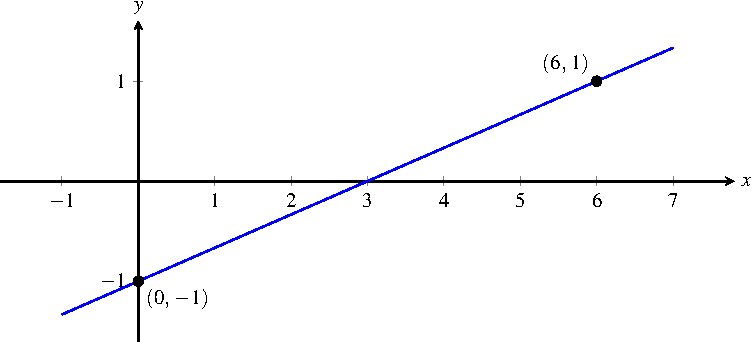
\includegraphics[scale=1]{image/06/thirdx-minus-3.pdf}
\caption{%%
  Two points on the graph of a linear function.
}
\label{fig:third_x_minus_3}
\end{figure}

\begin{exercise}
\Figure{fig:third_x_minus_3} shows the graph of a linear function
$f(x)$.  Use the information provided by the figure to construct the
function $f(x)$.
\end{exercise}
%%
\ifbool{showSolution}{
\begin{solution}
From \Figure{fig:third_x_minus_3}, you have the function values
$f(0) = -1$ and $f(6) = 1$.  The rate of change is
%%
\begin{align*}
a
&=
\frac{
  f(6) - f(0)
}{
  6 - 0
} \\[4pt]
&=
\frac{
  1 - (-1)
}{
  6
} \\[4pt]
&=
\frac{
  1 + 1
}{
  6
} \\[4pt]
&=
\frac{
  1
}{
  3
}.
\end{align*}
%%
Next, you calculate the $y$-intercept $\tuple{0}{b}$.  Using the value
$a = 1/3$ and the point $\tuple{0}{-1}$ from
\Figure{fig:third_x_minus_3}, you have the equation
$-1 = \frac{1}{3} \times 0 + b$.  The last equation simplifies to
$-1 = b$.  Therefore the graph in \Figure{fig:third_x_minus_3} can be
described by the linear function $f(x) = \frac{1}{3}x - 1$.
\end{solution}
}{}


%%%%%%%%%%%%%%%%%%%%%%%%%%%%%%%%%%%%%%%%%%%%%%%%%%%%%%%%%%%%%%%%%%%%%%%%%%%

\section{Intersection}

Consider two linear functions $f(x) = ax + b$ and $g(x) = cx + d$,
where the real numbers $\quadruple{a}{b}{c}{d}$ are known constants.
The graph of $f(x)$ can be represented by a straight line, call it
$\ell_1$, and the graph of $g(x)$ can be represented by another
straight line, call it $\ell_2$.  The lines $\ell_1$ and $\ell_2$ are
either parallel to each other or not parallel to each other.  If the
lines are parallel to each other, then the lines will never meet each
other.  In other words, there is no value of $x$ such that
$f(x) = g(x)$.  If $\ell_1$ and $\ell_2$ are not parallel to each
other, then the lines will intersect each other at one point.  This
means that there is a value of $x$ such that $f(x) = g(x)$.

To test whether the lines $\ell_1$ and $\ell_2$ intersect each other,
you equate $f(x)$ with $g(x)$ to get the expression $ax + b = cx + d$
and solve the latter expression for $x$.  This value of $x$,
e.g.~$x = x_1$, will be the $x$-coordinate of the point of
intersection.  Now substitute $x = x_1$ into the function $f(x)$~(or
$g(x)$, whichever looks easiest to work with) and simplify to
determine the $y$-coordinate of the point of intersection.  The above
description seems rather abstract.  The following examples should help
to clarify the points made above.

\begin{example}
\label{ex:intersection_2x_plus_1_x_plus_3}
Calculate the point of intersection of the functions $f(x) = 2x + 1$
and $g(x) = x + 3$.
\end{example}

\begin{solution}
Let $\ell_1$ and $\ell_2$ be the straight lines that represent the
functions $f(x)$ and $g(x)$, respectively.  The question assumes that
the lines $\ell_1$ and $\ell_2$ are not parallel to each other.  In
that case, there must exist a value $x = x_1$ such that
$f(x_1) = g(x_1)$.  Let's test this possibility.  First, you calculate
the $x$-coordinate of the point of intersection.  Equate the functions
$f(x)$ and $g(x)$ to obtain the expression $2x + 1 = x + 3$, which can
be written as $2x - x = 3 - 1$.  Simplify the latter expression to get
$x = 2$.  Now calculate the $y$-coordinate of the point of
intersection.  Substitute $x = 2$ into $g(x)$ to obtain $y = 2 + 3$
and simplifying results in $y = 5$.  As a check, you can also
substitute $x = 2$ into $f(x)$ to obtain $y = 2 \times 2 + 1$, which
also simplifies to $y = 5$.  Therefore the functions $f(x)$ and $g(x)$
intersect at the point $\tuple{2}{5}$ and so the straight lines that
represent these two functions are not parallel.
\end{solution}

\begin{exercise}
Let $\ell_1$ and $\ell_2$ be straight lines that represent the
functions $f(x)$ and $g(x)$, respectively, in
\Example{ex:intersection_2x_plus_1_x_plus_3}.  Explain another way to
help you decide whether the lines $\ell_1$ and $\ell_2$ intersect each
other.
\end{exercise}
%%
\ifbool{showSolution}{
\begin{solution}
Here is another way to help you decide whether the lines $\ell_1$ and
$\ell_2$ intersect each other.  On one set of coordinate axes you draw
the graphs of $f(x) = 2x + 1$ and $g(x) = x + 3$, as shown in
\Figure{fig:intersection_2x_plus_1_x_plus_3}.  From
\Figure{fig:intersection_2x_plus_1_x_plus_3}, you see that the graphs
of $f(x)$ and $g(x)$ intersect each other at one point.  Therefore you
conclude that the straight lines that represent $f(x)$ and $g(x)$ are
not parallel and has a point of intersection.

\begin{figure}[!htbp]
\centering
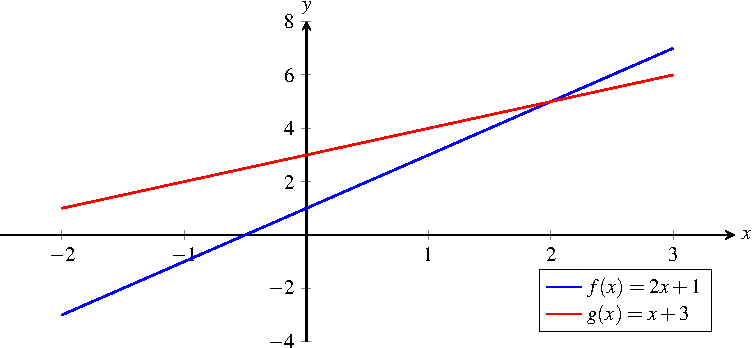
\includegraphics[scale=1]{image/06/2x+1_x+3.pdf}
\caption{%%
  A graph to help you decide whether the functions $f(x)$ and $g(x)$
  have a point of intersection.
}
\label{fig:intersection_2x_plus_1_x_plus_3}
\end{figure}
\end{solution}
}{}

\begin{example}
\label{ex:3x_plus_1_3x_plus_2}
Prove that the straight lines representing the linear functions
$f(x) = 3x + 1$ and $g(x) = 3x + 2$ are parallel to each other.
\end{example}

\begin{solution}
Let $\ell_1$ and $\ell_2$ be the straight lines that represent the
functions $f(x)$ and $g(x)$, respectively.  If $\ell_1$ and $\ell_2$
are parallel lines, then there is no value of $x$ such that
$f(x) = g(x)$.  To prove that $\ell_1$ and $\ell_2$ are parallel
lines, you may assume that they are not parallel and derive a
contradiction.  Let's assume that $\ell_1$ and $\ell_2$ are not
parallel.  Then there is a value of $x$ such that $f(x) = g(x)$.  To
compute the $x$-coordinate of the point of intersection, equate $f(x)$
and $g(x)$ to get $3x + 1 = 3x + 2$.  The last expression can be
written as $3x - 3x = 2 - 1$, which simplifies to $0 = 1$.  The
expression $0 = 1$ is a contradiction because zero and one are
different numbers so they cannot be equal.  The contradiction arises
because you assumed that the lines representing $f(x)$ and $g(x)$
intersect at a point.  Since your assumption leads to a contradiction,
you conclude that $\ell_1$ and $\ell_2$ are parallel.
\end{solution}

\begin{exercise}
Let $f(x)$ and $g(x)$ be as in \Example{ex:3x_plus_1_3x_plus_2} and
consider the function $h(x) = 3x + 3$.  Prove that the straight lines
that represent the functions $f(x)$, $g(x)$, and $h(x)$ are parallel
to each other.
\end{exercise}
%%
\ifbool{showSolution}{
\begin{solution}
Let $\triple{\ell_1}{\ell_2}{\ell_3}$ be straight lines that represent
the graphs of the functions $\triple{f(x)}{g(x)}{h(x)}$,
respectively.  You have three cases to consider.
%%
\begin{packedenumeral}
\item\label{case:ell1_ell2_parallel}
  Prove that $\ell_1$ and $\ell_2$ are parallel.

\item\label{case:ell1_ell3_parallel}
  Prove that $\ell_1$ and $\ell_3$ are parallel.

\item\label{case:ell2_ell3_parallel}
  Prove that $\ell_2$ and $\ell_3$ are parallel.
\end{packedenumeral}
%%
The solution to \Example{ex:3x_plus_1_3x_plus_2} proves
\Case{case:ell1_ell2_parallel}.  To prove
\Case{case:ell1_ell3_parallel}, you use the same argument as in
\Example{ex:3x_plus_1_3x_plus_2} by assuming that $\ell_1$ and
$\ell_3$ are not parallel and attempt to calculate a point of
intersection.  Equating the functions $f(x)$ and $h(x)$ results in the
expression $3x + 1 = 3x + 3$, which can be written as
$3x - 3x = 3 - 1$ and simplifies to $0 = 2$.  The contradiction
$0 = 2$ arises because you assumed that $f(x)$ and $h(x)$ has a point
of intersection.  Therefore $\ell_1$ and $\ell_3$ are parallel lines.

You now use the same argument as above to prove
\Case{case:ell2_ell3_parallel}.  Assume for contradiction that
$\ell_2$ and $\ell_3$ are not parallel.  Then the functions $g(x)$ and
$h(x)$ must have a point of intersection.  Equating $g(x)$ and $h(x)$
results in the expression $3x + 2 = 3x + 3$, which you can also write
as $3x - 3x = 3 - 2$ and simplify to $0 = 1$.  The contradiction
$0 = 1$ comes about because you assumed that the functions $g(x)$ and
$h(x)$ has a point of intersection.  Conclude that $\ell_2$ and
$\ell_3$ are parallel lines and therefore the straight lines
$\triple{\ell_1}{\ell_2}{\ell_3}$ are parallel to each other.
\end{solution}
}{}


\newpage
%%%%%%%%%%%%%%%%%%%%%%%%%%%%%%%%%%%%%%%%%%%%%%%%%%%%%%%%%%%%%%%%%%%%%%%%%%%

\section*{Problem}

\begin{problem}
\item Let $\quadruple{x_1}{x_2}{y_1}{y_2}$ be real numbers such that
  $x_1 < x_2$.  Consider the two points $A = \tuple{x_1}{y_1}$ and
  $B = \tuple{x_2}{y_2}$ in the Cartesian coordinate system.
  Determine a linear function of the form $f(x) = ax + b$ that passes
  through the points $A$ and $B$.  That is, calculate the values of
  the constants $a$ and $b$.
\ifbool{showSolution}{
\begin{solution}
You have the known values of $f(x_1) = y_1$ and $f(x_2) = y_2$.  Use
\Equation{eqn:linear_function_rate_of_change} to write the rate of
change as
%%
\begin{equation}
\label{eqn:derive_rate_of_change}
\begin{aligned}
a
&=
\frac{
  f(x_2) - f(x_1)
}{
  x_2 - x_1
} \\[4pt]
&=
\frac{
  y_2 - y_1
}{
  x_2 - x_1
}
\end{aligned}
\end{equation}
%%
To calculate the value of $b$, set $x = x_1$ so that $f(x_1) = y_1$.
Use the known value of $a$ to write the equation
$y_1 = ax_1 + b$, which can be solved for $b$ to produce
$b = y_1 - ax_1$ with $a$ as given in
\Equation{eqn:derive_rate_of_change}.
\end{solution}
}{}

\item Going anti-clockwise, there is a span of $\degree{45}$ from the
  positive half of the $x$-axis to the point $A = \tuple{1}{1}$.
  There is a span of $\degree{135}$ from the positive half of the
  $x$-axis to the point $B = \tuple{-1}{1}$, also going
  anti-clockwise.  Let $f(x) = a_1x + b_1$ be a function that passes
  through the point $A$.  Let $g(x) = a_2x + b_2$ be a function that
  passes through the point $B$ such that the straight lines in the
  graphs of $f(x)$ and $g(x)$ are perpendicular to each other.
  Determine two linear functions $f(x)$ and $g(x)$ that satisfy the
  above conditions.
\ifbool{showSolution}{
\begin{solution}
The points $A$ and $B$ are shown in
\Figure{fig:two_points_reflection_each_other_y_axis}, from which you
see that the line segments $OA$ and $OB$ are perpendicular to each
other.  All that you need to do now is to determine a linear function
$f(x)$ that goes through the origin $O$ and the point $A$, and another
linear function $g(x)$ that goes through the origin and the point
$B$.  Note that both linear functions will have the same
$y$-intercept, i.e.~the origin $\tuple{0}{0}$ itself.  Use
\Equation{eqn:derive_rate_of_change} to see that the rate of change of
$f(x)$ is given by
%%
\begin{align*}
a_1
&=
\frac{
  f(1) - f(0)
}{
  1 - 0
} \\[4pt]
&=
\frac{
  1 - 0
}{
  1 - 0
} \\[4pt]
&=
\frac{1}{1} \\[4pt]
&=
1.
\end{align*}
%%
Similarly, the rate of change of $g(x)$ is
%%
\begin{align*}
a_2
&=
\frac{
  g(-1) - g(0)
}{
  -1 - 0
} \\[4pt]
&=
\frac{
  1 - 0
}{
  -1 - 0
} \\[4pt]
&=
\frac{1}{-1} \\[4pt]
&=
-1.
\end{align*}
%%
Therefore the required linear functions are $f(x) = x$ and
$g(x) = -x$.

\begin{figure}[!htbp]
\centering
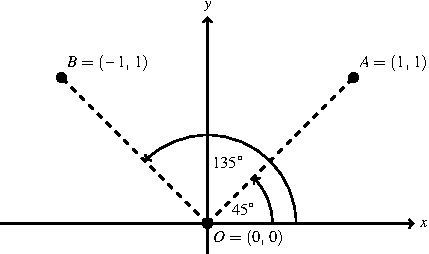
\includegraphics[scale=1.5]{image/06/perpendicular-lines-origin.pdf}
\caption{%%
  Two points that are reflections of each other with respect to the
  $y$-axis.  The angle from the line segment $OA$ to the segment $OB$
  is $\degree{135} - \degree{45} = \degree{90}$, going
  anti-clockwise.  Thus the segments $OA$ and $OB$ are perpendicular
  to each other.
}
\label{fig:two_points_reflection_each_other_y_axis}
\end{figure}
\end{solution}
}{}

\begin{table}[!htbp]
\centering
\begin{tabular}{cc} \toprule
Celsius $C$  & Fahrenheit $F(C)$ \\\midrule
$10$ & $50$ \\
$15$ & $59$ \\
$20$ & $68$ \\
$25$ & $77$ \\
$30$ & $86$ \\
$35$ & $95$ \\\bottomrule
\end{tabular}

\caption{%%
  Temperature conversion from degree Celsius to degree Fahrenheit.
}
\label{tab:temperature_Celsius_to_Fahrenheit}
\end{table}

\item \Table{tab:temperature_Celsius_to_Fahrenheit} shows how to
  convert between degrees Celsius and Fahrenheit.  Assume that the
  conversion from Celsius to Fahrenheit is given by a linear function
  of the form $F(C) = aC + b$, where $C$ represents the degree in
  Celsius and $F(C)$ represents the degree in Fahrenheit.  Determine
  the values of the constants $a$ and $b$.
\ifbool{showSolution}{
\begin{solution}
First, determine the rate of change.
\Table{tab:temperature_Celsius_to_Fahrenheit} shows that $F(10) = 50$
and $F(15) = 59$.  Use \Equation{eqn:linear_function_rate_of_change}
to write the rate of change as
%%
\begin{align*}
a
&=
\frac{
  F(15) - F(10)
}{
  15 - 10
} \\[4pt]
&=
\frac{
  59 - 50
}{
  15 - 10
} \\[4pt]
&=
\frac{9}{5}.
\end{align*}
%%
Next, determine the value of $b$.  Set $C = 10$ to get $F(10) = 50$.
Use the value of $a$ to write $50 = \frac{9}{5} \times 10 + b$, which
you can simplify to $50 = 9 \times 2 + b$ or $50 = 18 + b$.  Solving
the last equation for $b$ shows that $b = 50 - 18 = 32$.  Therefore
the conversion from degree Celsius to degree Fahrenheit is given by
the linear function $F(C) = \frac{9}{5} C + 32$.
\end{solution}
}{}

\begin{table}[!htbp]
\centering
\begin{tabular}{rc} \toprule
$x$  & $f(x)$ \\\midrule
$0$  & $1$    \\[6pt]
$1$  & $3$    \\[6pt]
$4$  & $5$    \\[6pt]
$9$  & $7$    \\[6pt]
$16$ & $9$    \\\bottomrule
\end{tabular}

\caption{%%
  Some values of an unknown function $f(x)$.  Is the function $f(x)$
  linear?
}
\label{tab:non_linear_function}
\end{table}

\item \Table{tab:non_linear_function} shows some values of a function
  $f(x)$.  You do not know a formula for $f(x)$.  However, you want to
  know whether the function $f(x)$ is linear.  Explain two different
  ways to help you decide whether $f(x)$ is linear.
\ifbool{showSolution}{
\begin{solution}
Suppose the values in \Table{tab:non_linear_function} are generated by
a function $f(x)$.  One way to decide whether the function $f(x)$ is
linear is to sketch the given points on one set of coordinate axes.
See \Figure{fig:plot_non_linear_function}.  If $f(x)$ is linear, you
would expect its graph to be one straight line going through the five
points given in \Table{tab:non_linear_function}.  However,
\Figure{fig:plot_non_linear_function} shows that the given points can
be joined up by multiple straight lines.  So from
\Figure{fig:plot_non_linear_function} you may conclude that the values
in \Table{tab:non_linear_function} are generated by a function that is
not linear.

To be absolutely sure that the function $f(x)$ is not linear, you can
use \Equation{eqn:linear_function_rate_of_change} to calculate the
rate of change for two different pairs of points.  If $f(x)$ is
linear, you would expect $f(x)$ to have exactly one rate of change.
Let's calculate the rate of change by using the points $\tuple{0}{1}$
and $\tuple{1}{3}$.  These two points result in the rate of change
%%
\begin{align*}
\frac{
  f(1) - f(0)
}{
  1 - 0
}
&=
\frac{
  3 - 1
}{
  1
} \\[4pt]
&=
\frac{
  2
}{
  1
} \\[4pt]
&=
2.
\end{align*}
%%
Let's calculate the rate of change by using the different points
$\tuple{4}{5}$ and $\tuple{9}{7}$.  The latter pair of points results
in the rate of change
%%
\begin{align*}
\frac{
  f(9) - f(4)
}{
  9 - 4
}
&=
\frac{
  7 - 5
}{
  5
} \\[4pt]
&=
\frac{
  2
}{
  5
}
\end{align*}
%%
which is different from the rate of $2$ that you calculated above.
Therefore the function $f(x)$ that generated the data in
\Table{tab:non_linear_function} is not linear.

\begin{figure}[!htbp]
\centering
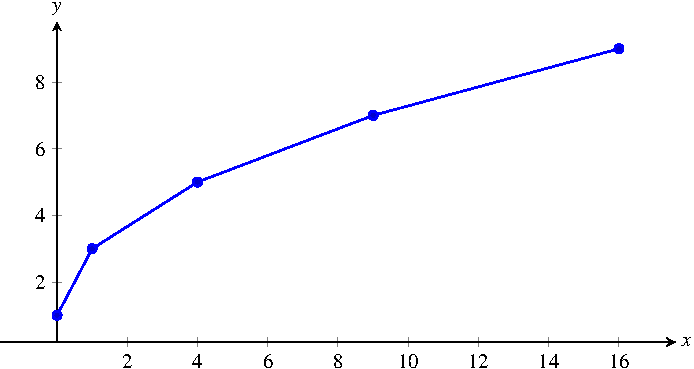
\includegraphics[scale=1]{image/06/nonlinear.pdf}
\caption{%%
  A plot of the data points from \Table{tab:non_linear_function}.
}
\label{fig:plot_non_linear_function}
\end{figure}
\end{solution}
}{}

\item Consider the functions $f(x) = ax + b$ and $g(x) = ax + c$,
  where the real numbers $\triple{a}{b}{c}$ are known constants such
  that $b \neq c$.  Prove that the straight lines that represent the
  graphs of $f(x)$ and $g(x)$ are parallel to each other.
\ifbool{showSolution}{
\begin{solution}
Let $\ell_1$ and $\ell_2$ be straight lines that represent the graphs
of $f(x)$ and $g(x)$, respectively.  To prove that $\ell_1$ and
$\ell_2$ are parallel lines, assume for contradiction that they are
not parallel and attempt to derive a point at which the graphs of
$f(x)$ and $g(x)$ intersect each other.  Equating $f(x)$ and $g(x)$
shows that you have the expression $ax + b = ax + c$, which you can
also write as $ax - ax = c - b$.  The last expression simplifies to
$0 = c - b$.  Since you have assumed that $b \neq c$, their difference
cannot be zero and so $c - b \neq 0$.  In other words, the expression
$0 = c - b$ is a contradiction, which arises because you assumed that
$f(x)$ and $g(x)$ has a point of intersection.  Conclude that $f(x)$
and $g(x)$ do not have a point of intersection and therefore the lines
$\pair{\ell_1}{\ell_2}$ are parallel to each other.
\end{solution}
}{}

\item\label{prob:linear_functions_intersection_point}
  Let $\quadruple{a}{b}{c}{d} \in \RR$ be known constants.
  Consider the linear functions $f(x) = ax + b$ and $g(x) = cx + d$.
  %%
  \begin{packedenum}
  \item\label{subprob:intersection_point_x_y_coordinates}
    Suppose that the functions $f(x)$ and $g(x)$ have a point of
    intersection.  Prove that the $x$-coordinate of the point of
    intersection is
    %%
    \begin{equation}
    \label{eqn:intersection_point_x_coordinate}
    x
    =
    \frac{d - b}{a - c}
    \end{equation}
    %%
    and the $y$-coordinate of the point of intersection is
    \[
    y
    =
    \frac{a(d - b)}{a - c}
    +
    b.
    \]

  \item\label{subprob:intersection_point_undefined}
    For which values of $a$ and $c$ would
    \Equation{eqn:intersection_point_x_coordinate} not make sense?
    Explain why \Equation{eqn:intersection_point_x_coordinate} would
    not make sense for those particular values of $a$ and $c$.

  \item\label{subprob:intersection_point_on_y_axis}
    Suppose that $a \neq c$ and $d = b$.  Where would you expect to
    find the point at which $f(x)$ and $g(x)$ intersect each other?

  \item\label{subprob:intersection_point_on_x_axis}
    Suppose that $a \neq c$ and $b = ad / c$.  Where would you expect
    to find the point at which $f(x)$ and $g(x)$ intersect each other?

  \item\label{subprob:intersection_point_origin}
    Suppose that $a \neq c$ and $b = d = 0$.  Prove that $f(x)$ and
    $g(x)$ intersect each other at the origin.
  \end{packedenum}
\ifbool{showSolution}{
\begin{solution}
\solutionpart{subprob:intersection_point_x_y_coordinates}
To determine the coordinates of the point at which $f(x)$ and $g(x)$
intersect each other, you equate $f(x)$ and $g(x)$ to obtain the
expression $ax + b = cx + d$.  Write the last expression as
$ax - cx = d - b$, which can be factored as
$x(a - c) = d - b$ and solving for $x$ results in
\[
x
=
\frac{d - b}{a - c}.
\]
This is the same as \Equation{eqn:intersection_point_x_coordinate}.
To determine the $y$-coordinate of the point of intersection,
substitute \Equation{eqn:intersection_point_x_coordinate} into
$f(x) = ax + b$ to obtain
%%
\begin{align*}
y
&=
a \times \frac{d - b}{a - c} + b \\[4pt]
&=
\frac{a(d - b)}{a - c} + b.
\end{align*}

\solutionpart{subprob:intersection_point_undefined}
Equation~\eqref{eqn:intersection_point_x_coordinate} does not make
sense whenever $a = c$.  This is because $a = c$ would mean that
$a - c = 0$ and dividing by zero is undefined.

\solutionpart{subprob:intersection_point_on_y_axis}
If $a \neq c$ but $d = b$, then
\Equation{eqn:intersection_point_x_coordinate} becomes $x = 0$ and the
$y$-coordinate of the point of intersection is $y = b$.  Thus the
point of intersection is $\tuple{0}{b}$ so you would expect to find
the intersection point on the $y$-axis.

\solutionpart{subprob:intersection_point_on_x_axis}
If $a \neq c$ but $b = ad / c$, then
\Equation{eqn:intersection_point_x_coordinate} can be written as
%%
\begin{align*}
x
&=
\frac{d}{a - c} - \frac{b}{a - c} \\[4pt]
&=
\frac{d}{a - c} - \frac{ad / c}{a - c} \\[4pt]
&=
\frac{d}{a - c} - \frac{ad}{c} \times \frac{1}{a - c} \\[4pt]
&=
\frac{cd}{c(a - c)} - \frac{ad}{c(a - c)} \\[4pt]
&=
\frac{d(c - a)}{c(a - c)} \\[4pt]
&=
-\frac{d(a - c)}{c(a - c)} \\[4pt]
&=
-\frac{d}{c}.
\end{align*}
%%
The $y$-coordinate of the point of intersection is
%%
\begin{align*}
y
&=
a \times \parenthesis*{-\frac{d}{c}} + \frac{ad}{c} \\[4pt]
&=
-\frac{ad}{c} + \frac{ad}{c} \\[4pt]
&=
0.
\end{align*}
%%
Thus the point of intersection is $\tuple{-\frac{d}{c}}{0}$ and so you
would expect to find the intersection point on the $x$-axis.

\solutionpart{subprob:intersection_point_origin}
If $b = d = 0$, then $d - b = 0$.
From \Part{subprob:intersection_point_x_y_coordinates} the $x$- and
$y$-coordinates of the point of intersection are $x = 0$ and $y = 0$,
respectively.  In other words, the functions $f(x)$ and $g(x)$
intersect each other at the origin $\tuple{0}{0}$.
\end{solution}
}{}

\begin{table}[!htbp]
\centering
\begin{tabular}{cc} \toprule
Age  & Height \\\midrule
$10$ & $1.38$ \\
$11$ & $1.44$ \\
$12$ & $1.50$ \\
$13$ & $1.56$ \\
$14$ & $1.62$ \\
$15$ & $1.68$ \\\bottomrule
\end{tabular}

\caption{%%
  The height of a child between the ages of $10$ and $15$.  Age is
  measured in years and height is measured in metres.
}
\label{tab:children_height_by_age}
\end{table}

\item \Table{tab:children_height_by_age} tracks the height~(in metres)
  of a child from when the child was ten years old to the age of $15$
  years old.  Suppose that during the ages of ten to $15$ years old,
  the child grew at a constant rate of $a$.  Let $x$ be the age~(in
  years) of the child.  Suppose that the height of the child can be
  written as a linear function of the form $h(x) = ax + b$.
  %%
  \begin{packedenum}
  \item\label{subprob:height_function_rate_of_change}
    Use \Table{tab:children_height_by_age} to calculate the rate $a$.
    Explain the rate $a$ in terms of the height of the child.

  \item\label{subprob:height_function_y_intercept}
    Calculate the value of $b$.  Explain this value in terms of the
    child's height.

  \item\label{subprob:height_function_height_at_20_30}
    Use your solutions
    from \Parts{subprob:height_function_rate_of_change}{subprob:height_function_y_intercept}
    to recover the function $h(x)$.  Use the function $h(x)$ to
    calculate the child's height when the child is $20$ years old.
    Again use the function $h(x)$ to determine the child's height at
    $30$ years old.  Explain what is wrong with the two heights you
    obtained.
  \end{packedenum}
\ifbool{showSolution}{
\begin{solution}
\solutionpart{subprob:height_function_rate_of_change}
From \Table{tab:children_height_by_age} you have the function values
$h(10) = 1.38$ and $h(11) = 1.44$.  The rate of change is
%%
\begin{align*}
a
&=
\frac{
  h(11) - h(10)
}{
  11 - 10
} \\[4pt]
&=
\frac{
  1.44 - 1.38
}{
  1
} \\[4pt]
&=
\frac{
  0.06
}{
  1
} \\[4pt]
&=
0.06.
\end{align*}
%%
The rate $a = 0.06$ means that each year the child grew by $0.06$
metres.  In other words, the child grew by $6$~cm per year.

\solutionpart{subprob:height_function_y_intercept}
You can use the function value $f(10) = 1.38$ to calculate the value
of $b$.  Using the value $a = 0.06$ results in the expression
$1.38 = 0.06 \times 10 + b$, which simplifies to $1.38 = 0.6 + b$.
Solving the latter expression for $b$ to obtain
$b = 1.38 - 0.6 = 0.78$.  Note that in the expression
$h(x) = ax + b$, if $x = 0$ then you have $h(0) = b$.  In other words,
the value $b = 0.78$ means that when the child was born~(zero years
old) the height at birth was $b = 0.78$ metres~(or $78$~cm).

\solutionpart{subprob:height_function_height_at_20_30}
From \Parts{subprob:height_function_rate_of_change}{subprob:height_function_y_intercept},
the height function can be written as $h(x) = 0.06x + 0.78$.  At the
age of $x = 20$ years old, the child will be $h(20) = 1.98$ metres
tall.  At the age of $x = 30$ years old, the child will be
$h(30) = 2.58$ metres tall.  These two height numbers do not make
sense because a human being usually stops getting taller after a
certain age.  In other words, the height function $h(x)$ is only valid
within a particular age range.  In the case of
\Table{tab:children_height_by_age}, the function $h(x)$ is valid
between the ages of $10$ and $15$ years old, inclusive.  Below ten
years old~(or after $15$ years old), the function $h(x)$ can give a
ridiculous height value.
\end{solution}
}{}

\begin{figure}[!htbp]
\centering
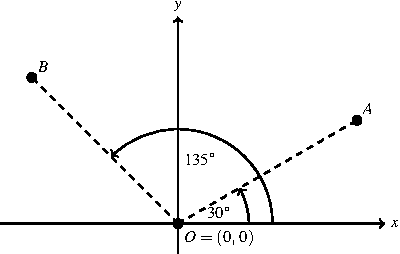
\includegraphics[scale=1.5]{image/06/points-unit-circle.pdf}
\caption{%%
  An ant starts at point $A$ and travels along a straight line to
  point $B$.  Both points lie on the same unit circle that is centred
  at the origin.
}
\label{fig:unit_circle_A_30_degrees_B_135_degrees}
\end{figure}

\item The positions of an ant are illustrated in
  \Figure{fig:unit_circle_A_30_degrees_B_135_degrees}.  The ant starts
  at point $A$ and travels along a straight line to point $B$.
  Suppose that the time required for the ant to reach its destination
  $B$ is measured in seconds and the distance between $A$ and $B$ is
  measured in metres.  Assume that both $A$ and $B$ lie on the unit
  circle centred at the origin.
  %%
  \begin{packedenum}
  \item\label{subprob:ant_coordinates_of_points}
    Calculate the Cartesian coordinates of the point $A$.  Do the same
    for the point $B$.

  \item\label{subprob:ant_distance_travelled}
    Calculate the distance that the ant travelled.

  \item\label{subprob:ant_rate_per_second}
    Calculate the rate~(in metres per second) at which the ant
    travelled from $A$ to $B$.

  \item\label{subprob:ant_how_long_to_destination}
    How long~(in seconds) did the ant take to travel from $A$ to $B$?
  \end{packedenum}
\ifbool{showSolution}{
\begin{solution}
\solutionpart{subprob:ant_coordinates_of_points}
The point $A$ makes an angle of $\degree{30}$~(or $\pi / 6$ radians)
with respect to the positive half of the $x$-axis.  Since $A$ lies on
the unit circle centred at the origin, the circle has a radius of $1$
and so $A$ can be described by the polar coordinates
$\tuple{1}{\frac{\pi}{6}}$.  In the Cartesian coordinate system, the
$x$-coordinate of $A$ is
%%
\begin{align*}
x
&=
\cos\frac{\pi}{6} \\[4pt]
&=
\frac{\sqrt{3}}{2}
\end{align*}
%%
and the $y$-coordinate of $A$ is
%%
\begin{align*}
y
&=
\sin\frac{\pi}{6} \\[4pt]
&=
\frac{1}{2}.
\end{align*}
%%
The Cartesian coordinates of $A$ are
$\tuple{\frac{\sqrt{3}}{2}}{\frac{1}{2}}$.

Similarly, the point $B$ can be described by the polar coordinates
$\tuple{1}{\frac{3\pi}{4}}$ because $\degree{135}$ is equivalent to
$\frac{3\pi}{4}$ radians.  The $x$-coordinate of $B$ is
%%
\begin{align*}
x
&=
\cos\frac{3\pi}{4} \\[4pt]
&=
-\frac{\sqrt{2}}{2}
\end{align*}
%%
and the $y$-coordinate of $B$ is
%%
\begin{align*}
y
&=
\sin\frac{3\pi}{4} \\[4pt]
&=
\frac{\sqrt{2}}{2}.
\end{align*}
%%
Thus $B$ has the Cartesian coordinates
$\tuple{-\frac{\sqrt{2}}{2}}{\frac{\sqrt{2}}{2}}$.

\solutionpart{subprob:ant_distance_travelled}
The distance $d$ between points $A$ and $B$ can be calculated as
%%
\begin{align*}
d
&=
\sqrt{
  \parenthesis*{
    \frac{\sqrt{2}}{2} - \frac{1}{2}
  }^2
  +
  \parenthesis*{
    -\frac{\sqrt{2}}{2} - \frac{\sqrt{3}}{2}
  }^2
} \\[4pt]
&=
\sqrt{
  \parenthesis*{
    \frac{\sqrt{2} - 1}{2}
  }^2
  +
  \parenthesis*{
    -
    \parenthesis*{
      \frac{\sqrt{2}}{2} + \frac{\sqrt{3}}{2}
    }
  }^2
} \\[4pt]
&=
\sqrt{
  \parenthesis*{
    \frac{\sqrt{2} - 1}{2}
  }^2
  +
  \parenthesis*{
    - \frac{\sqrt{2} + \sqrt{3}}{2}
  }^2
} \\[4pt]
&=
\sqrt{
  \frac{3 - 2\sqrt{2}}{4}
  +
  \frac{5 + 2\sqrt{6}}{4}
} \\[4pt]
&=
\sqrt{
  \frac{
    2\sqrt{6} - 2\sqrt{2} + 8
  }{
    4
  }
} \\[4pt]
&=
\frac{1}{2}
\sqrt{
  2\sqrt{6} - 2\sqrt{2} + 8
}.
\end{align*}
%%
The ant travelled approximately $d \approx 1.586707$ metres, rounded to
six decimal places.

\solutionpart{subprob:ant_rate_per_second}
Since the ant is assumed to travel in a straight line from $A$ to $B$,
the rate in metres per second at which the ant travelled can be
obtained by first calculating the rate of change $a$ in the linear
function $f(x) = ax + b$.  Here, you want the function $f(x)$ to pass
through the points $A$ and $B$.  Using the Cartesian coordinates of
the points $A$ and $B$, the rate of change $a$ is given by
%%
\begin{align*}
a
&=
\frac{
  \frac{\sqrt{2}}{2} - \frac{1}{2}
}{
  -\frac{\sqrt{2}}{2} - \frac{\sqrt{3}}{2}
} \\[4pt]
&=
\frac{
  -\frac{1}{4} \sqrt{2} (\sqrt{2} - 2)
}{
  -\frac{1}{4} \sqrt{2} (\sqrt{6} + 2)
} \\[4pt]
&=
\frac{
  \sqrt{2} - 2
}{
  \sqrt{6} + 2
}.
\end{align*}
%%
Note that $a < 0$ because the numerator $\sqrt{2} - 2 < 0$.  To
convert $a$ to the rate at which the ant travelled, you take the
absolute value of $a$.  Thus the ant travelled at a rate of
approximately $\absoluteValue{a} \approx 0.131652$ metres per second,
rounded to six decimal places.

\solutionpart{subprob:ant_how_long_to_destination}
The time $t$ in seconds that the ant took to travel from $A$ to $B$
can be obtained by dividing the distance travelled by the rate of
travel.  Using the approximate values of distance and rate
in \Parts{subprob:ant_distance_travelled}{subprob:ant_rate_per_second},
you can estimate the time required as
\[
t
\approx
\frac{1.586707}{0.131652}.
\]
In other words, the ant took approximately $t \approx 12.05$ seconds
to travel from $A$ to $B$, rounded to two decimal places.
\end{solution}
}{}

\item Two animals $A$ and $B$ are running in a straight line along the
  same direction.  Initially, animal $A$ was $3$ metres ahead of
  animal $B$.  Animal $A$ runs at a constant rate of $2$ metres per
  second and $B$ runs at a rate of $2.5$ metres per second.
  %%
  \begin{packedenum}
  \item\label{subprob:rat_race_linear_functions}
    Let $f(t)$ and $g(t)$ be the distances in metres that animals $A$
    and $B$ have travelled, respectively, after $t$ seconds.
    Construct the functions $f(t)$ and $g(t)$.  Graph the functions on
    the same set of coordinate axes from $t = 0$ to $t = 8$ seconds.

  \item\label{subprob:rat_race_catch_up}
    How long~(in seconds) does animal $B$ take to catch up to $A$?
    When both animals meet, how far~(in metres) would each animal have
    travelled?

  \item\label{subprob:rat_race_any_head_start}
    Suppose that animal $A$ is initially $s$ metres ahead of $B$,
    where $s > 0$ is any real number.  Explain why $B$ would
    eventually catch up to $A$.
  \end{packedenum}
\ifbool{showSolution}{
\begin{solution}
\solutionpart{subprob:rat_race_linear_functions}
Suppose the function $f(t)$ is a linear function of the form
$f(t) = at + b$.  At time $t = 0$, animal $A$ is $3$ metres ahead of
$B$ so the $y$-intercept is $\tuple{0}{3}$ and hence $b = 3$.  Since
$A$ runs at a constant rate of $2$ metres per second, then you have
$a = 2$.  The function $f(t)$ can now be written as
$f(t) = 2t + 3$.  You can use the same argument as above to construct
the function $g(t)$.  First, you assume that $g(t)$ is a linear
function of the form $g(t) = ct + d$.  At time $t = 0$, animal $B$ has
not covered any amount of distance so $g(t) = 0$ and the $y$-intercept
is $d = 0$.  You also have $c = 2.5$ because $B$ runs at a constant
rate of $2.5$ metres per second.  In other words, the function $g(t)$
can be written as $g(t) = 2.5t$.  See
\Figure{fig:distances_as_functions_of_time} for the graphs of the
above two functions.

\begin{figure}[!htbp]
\centering
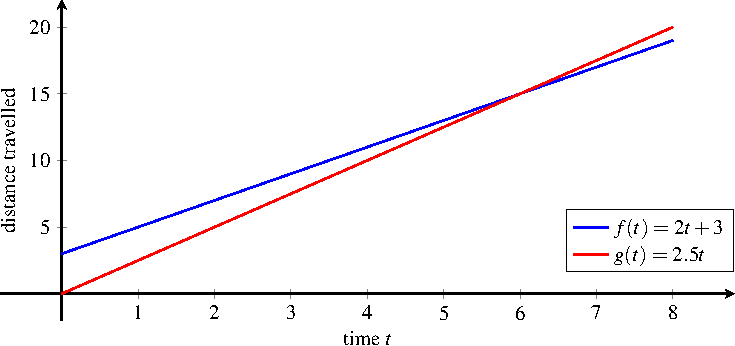
\includegraphics[scale=1]{image/06/rat-race.pdf}
\caption{%%
  The distances that the animals $A$ and $B$ travelled as functions of
  time.  Time is measured in seconds and distance is measured in
  metres.  The distance functions of $A$ and $B$ are $f(t)$ and
  $g(t)$, respectively.
}
\label{fig:distances_as_functions_of_time}
\end{figure}

\solutionpart{subprob:rat_race_catch_up}
The point of intersection of the functions $f(t)$ and $g(t)$ should
give you the time and distance at which the animals meet each other.
Equate $f(t)$ and $g(t)$ to obtain the expression $2t + 3 = 2.5t$,
which can be written as $2.5t - 2t = 3$ and simplified to
$0.5t = 3$ or $\frac{1}{2}t = 3$.  Solving the last expression for $t$
shows that animal $B$ catches up to animal $A$ after
$t = 3 \times 2 = 6$ seconds.  Now let's calculate the distance that
both animals would have travelled after six seconds.  Substitute
$t = 6$ into the expression $f(t) = 2t + 3$ to get
$f(6) = 2 \times 6 + 3$, which can be simplified to $f(6) = 12 + 3$ or
$f(6) = 15$.  After $t = 6$ seconds, animal $B$ would have caught up
to $A$ and each animal would have covered $15$ metres.

\solutionpart{subprob:rat_race_any_head_start}
Suppose that $A$ is initially $s > 0$ metres ahead of $B$.  The
distance function of $B$ is still $g(t) = 2.5t$, but the distance
function of $A$ is now $f(t) = 2t + s$.  Since both animals run at
different rates, you may
use \Parts{subprob:intersection_point_x_y_coordinates}{subprob:intersection_point_undefined}
of \Problem{prob:linear_functions_intersection_point} to conclude that
both animals will eventually meet each other.  The time at which the
animals meet each other can be calculated as follows.  Equate $f(t)$
and $g(t)$ to obtain the expression $2t + s = 2.5t$, which can be
written as $2.5t - 2t = s$ and simplified to $0.5t = s$ or
$\frac{1}{2} t = s$.  Solving the last equation for $t$ shows that
animal $B$ will eventually catch up to $A$ after $t = 2s$ seconds.
\end{solution}
}{}

\item Explain an example of a situation~(different from those
  presented in this document) that can be represented as a linear
  function.  Construct a linear function for your example.
\ifbool{showSolution}{
\begin{solution}
Here is a situation that can be represented as a linear function.
Water is dripping down into a bucket that was initially empty.  The
water drips at a constant rate of $0.1$ litres per second.  If time
$t$ is measured in seconds, then after $t$ seconds the bucket would
contain $f(t) = 0.1t$ litres of water.
\end{solution}
}{}
\end{problem}

\end{document}
